\section{What is MPS?}
\label{section:MPS}

Language workbenches (LWB) are a tool to help language engineers create languages, particularly domain-specific languages (DSL).
Fowler\cite{Fowler_lwb} popularised the term LWB in a 2005 article.

Meta Programming System (MPS) is an open-source LWB that assists in the creation of projectional languages.
It started in 2003 by JetBrains and was introduced to the world in Sergey Dmitriev's 2004 Paper ``Language Orientated Programming: the Next Programming Paradigm''\cite{dmitriev2004language}.

As discussed in section \ref{section:WhatIsPE}, when creating a projectional language, one must define the language and how one interacts with it.
In MPS, the language engineer defines languages, including their interactions.
Developers create programs using these languages.
The language engineer can extend languages.
The developer can mix the languages she uses.

The following is an overview of how MPS implements the ideal of a projectional language.
It is also the structure of this section: 

\begin{itemize}
    \setlength\itemsep{0em}
    \item Abstract syntax
    \begin{itemize}
        \setlength\itemsep{0em}
        \item Structure
        \item Behaviors\footnote{When referring to its use in the MPS workbench, consistent with their use, we use the American spelling - Behavior.}
        \item Constraints
        \item Type system
    \end{itemize}
    \item Concrete syntax
    \begin{itemize}
        \setlength\itemsep{0em}
        \item Editors
        \item Intentions
    \end{itemize}
    \item Generators
    \begin{itemize}
        \setlength\itemsep{0em}
        \item Model-to-Model
        \item Model-to-Text
    \end{itemize}
\end{itemize}

MPS defines the different aspects of the language definitions with small, declarative DSLs.
These are bundled together into what they term Aspects.

\subsection{Abstract Syntax: Structure}
Structure is what determines the abstract syntax of a language.
The most important item available in a Structure Aspect is the Concept.
Instances of concepts are called nodes.
With these nodes, the developers construct their programs.
When referring to a program in MPS, we are talking about its stored abstract syntax tree (AST).

In principle, a concept contains three types of things:
\begin{enumerate}
    \setlength\itemsep{0em}
    \item Properties: these primitives are integer, boolean, string, or enum items and are similar to leaf values.
    \item Children: these are other concepts, or collections of them, similar to subtrees.
    \item References: these are relationships with other nodes in the AST. These turn the tree into a graph.
\end{enumerate}

Concepts follow some object orientated (OO) traits, such as subtype, being abstract, and implementing interfaces.

One of these Concepts must be a root node. 
Otherwise, there is nowhere for a program to start.

Other items available in the Structure Aspect are the Interface Concept, the Enumeration, the Constrained Data Type, and the Primitive Datatype.
\footnote{At the time of writing, we are unaware whether Data Type and Datatype are semantically different or that the different naming is just a style choice.}

Thus, the Structure aspect defines how the AST can be structured.

Figure \ref{fig:concept_example} shows a concept with three children that implements two interfaces.
The first line names the concept and which concept it extends.
By default all concepts extend \texttt{BaseConcept}.
The next two lines shows the interfaces it implements.
This concept is not rootable, and therefore cannot be instantiated as a file in a solution.
the alias and short description override what will be shown in menus instead of \texttt{RuleStatement} and its fully qualitfied name.
This concept has no custom properties or references.
It has three children.
The attributes child contains one and only one RuleAttributes Concept.
Outcomes also contains only one child concept, this one of type StatementList.
The conditions child has a collection of abstract conditions

\begin{figure}[h]
    \centering
    \fbox{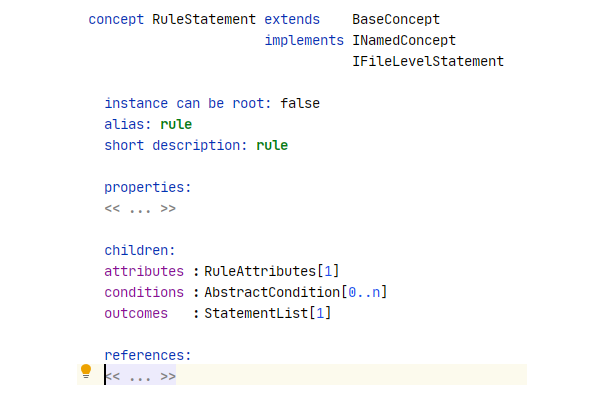
\includegraphics[width=0.66\textwidth]{Sections/images/concept_example_P.png}}
    \caption{Concept example}
    \label{fig:concept_example}
\end{figure}
 
\subsection{Abstract Syntax: Behaviors}
OO design usually bundles together data and methods that can act on that data.
Concepts are analogous to the data part of this equation.
Behavior fills the role of the methods in the OO analogy, defining the functionality called from instantiated nodes and static methods called from the Concept.
The Constructor is a specialised method in a Behavior, filling the same role as a constructor in OO.

The methods have public, private, or protected visibility.
If the Concept to which the Behavior refers is abstract, the Behavior itself can contain abstract methods.
Abstraction, variable visibility and inheritance allow a sort of polymorphism.
If a virtual method is declared, then it can be called polymorphically.

Figure \ref{fig:behavior_example} shows a constructor added to a Concept to initialise its children.
It has a method to allow other nodes to interrogate the condition of it having attributes.

\begin{figure}[h]
    \centering
    \fbox{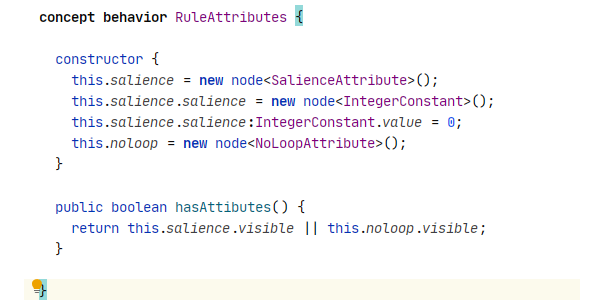
\includegraphics[width=0.66\textwidth]{Sections/images/behavior_example_P.png}}
    \caption{Behavior example}
    \label{fig:behavior_example}
\end{figure}

\newpage
\subsection{Abstract Syntax: Constraints}
A Constraints aspect adds further structural restrictions to a Concept.
Constraints primarily define scope by controlling if another node can be a child, a parent, or an ancestor of this node.
A Constraint can also prevent badly formed properties, children or references.

Figure \ref{fig:constraint_example} shows an example of a scope restraint that only allows local variables declared within the same rule or global variables declared in the same file.
 
\begin{figure}[h]
    \centering
    \fbox{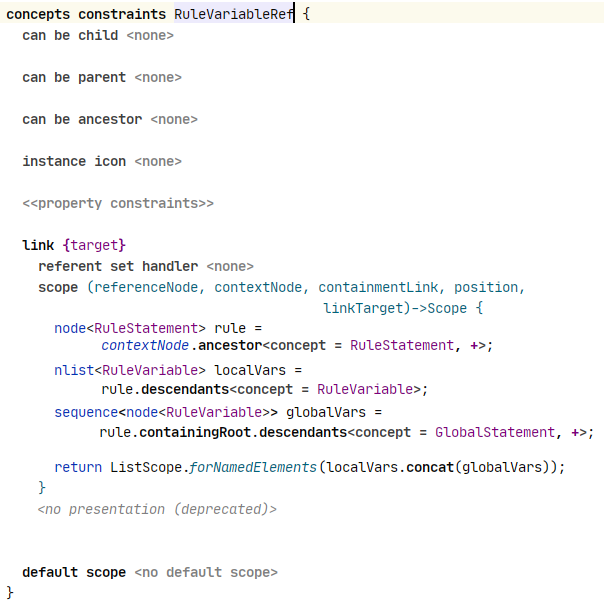
\includegraphics[width=0.66\textwidth]{Sections/images/constraint_example_P.png}}
    \caption{Constraint example}
    \label{fig:constraint_example}
\end{figure}

\subsection{Abstract Syntax: Type System}
The Type system aspect and the constraints aspect together represent the static semantics of the language.
This aspect is for the computation and evaluation of types of variables, expressions and statements.

Rules that are available to calculate and enforce the type system include inference, subtyping, comparison and substitute type rules.

Figure \ref{fig:typesystem_example} shows an inference rule that ensures that the calculated type of the import statement matched that of its child called type.

\begin{figure}[h]
    \centering
    \fbox{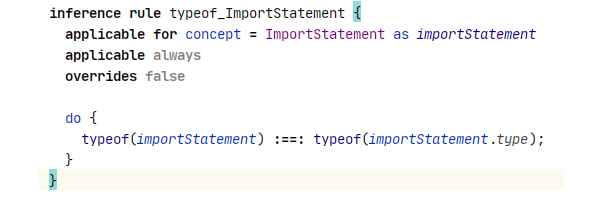
\includegraphics[width=0.66\textwidth]{Sections/images/typesystem_example_P.png}}
    \caption{Type system example}
    \label{fig:typesystem_example}
\end{figure}

\subsection{Concrete Syntax: Editors}
Editor aspects define the notation of the nodes.
In effect, it is the user interface of the language, projecting the AST to the developer.
An editor is a swing panel that renders a tree of editor cells.
A concept can have multiple editors, thus offering multiple views on it.

The definition of the options available to the developers through menus also happens within the Editor Aspect. 
The choice the developer makes transforms the existing AST.

Additionally, the behaviour of interactions can be defined, such as what will happen to the AST when a particular keypress or editor action occurs at a particular location.

Figure \ref{fig:editor_example} shows a component with a projection for the Concept shown in figure \ref{fig:concept_example}.

\begin{figure}[h]
    \centering
    \fbox{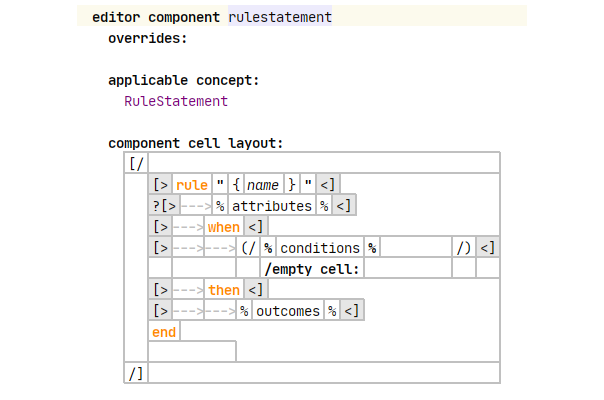
\includegraphics[width=0.66\textwidth]{Sections/images/editor_example_P.png}}
    \caption{Editor example}
    \label{fig:editor_example}
\end{figure}

\subsection{Concrete Syntax: Intentions}

In projectional editing, the IDE is a part of the concrete syntax.
Intentions make context-aware suggestions for automatic changes to the program to the developer.
Figure \ref{fig:intention_example} shows an intention that allows the developer to add, remove or edit a property based on its current value.

\begin{figure}[h]
    \centering
    \fbox{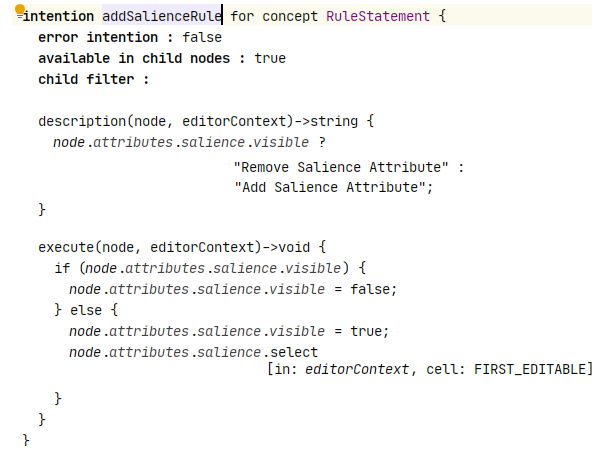
\includegraphics[width=0.66\textwidth]{Sections/images/intention_example_P.png}}
    \caption{Intention example}
    \label{fig:intention_example}
\end{figure}

\subsection{Generators}
In our implementation we will not be using generators.
However, as they are an important part of a typical language implementation, we will discuss them briefly here.

There are two types of generator, the Model-to-Text generator and the Model-to-Model generator.

Whilst designing a language is nice, it has to be able to do something. 
Without doing so, it has no semantic meaning.
It is possible to create interpreters that can use the AST generated by MPS.

However, the most common modality for MPS is to generate, via a model-to-text generator, an output that gets compiled and run by commonly known environments.
The output stage of generation is called TextGen.
It defines how a node becomes runnable code in plain text.

Base level languages will have text generation.
Most DSLs will perform model-to-model conversions, eventually converting to a base language.
These intermediate stages are known as Generator Aspects.
They transform code written in one language to another.

In MPS, a Concept can have multiple generators aimed at different base level languages, such as Java (using MPS BaseLanguage), C (using mbeddr) or XML.